\documentclass[parskip=full]{scrartcl}
\usepackage[utf8]{inputenc} % use utf8 file encoding for TeX sources
\usepackage[T1]{fontenc}    % avoid garbled Unicode text in pdf
\usepackage[german]{babel}  % german hyphenation, quotes, etc
\usepackage{graphicx}
\usepackage{rotating}
\graphicspath{ {images/} }
\usepackage{hyperref}       % detailed hyperlink/pdf configuration
\hypersetup{                % ‘texdoc hyperref‘ for options
pdftitle={PSE : DataMovementDeaon},%
bookmarks=true,%
}
\usepackage{graphicx}       % provides commands for including figures
\usepackage{csquotes}       % provides \enquote{} macro for "quotes"
\usepackage[nonumberlist, acronym]{glossaries} % provides glossary commands
\usepackage{enumitem}
\usepackage{lscape}
\usepackage{caption}
\usepackage{rotating}
\usepackage{placeins}

\makenoidxglossaries
%
%%Glossary
%
\newglossaryentry{generator}
{
	name=generator,
	plural=generators,
	description={The first module in the program. Responsible for generating artificial matrices and collection preexisting matrices from the suite sparse matrix collection.}
}

\newglossaryentry{labeling module}
{
	name=labeling module,
	plural=labeling module,
	description={The second module in the program. Responsible for executing a given set of matrices with all the preconditioner/iterative solvers combination specified. It will furthermore label each matrix with the fastest combination.}
}

\newglossaryentry{neural network}
{
	name=neural network,
	plural=neural networks,
	description={The third module in the program. Responsible for training a deep neural network with the set of matrices and labels given by the labeling module.}
}

\newglossaryentry{classifier}
{
	name=classifier,
	plural=classifier,
	description={The last and main module in the program.It is able to determine the fastest preconditioner/iterative solver combination for a given sparse linear system. It uses the neural network trained by the module neural network.}
}

\newglossaryentry{preconditioner}
{
	name=preconditioner,
	plural=preconditioners,
	description={WIP}
}

\newglossaryentry{iterative solver}
{
	name=iterative solver,
	plural=iterative solvers,
	description={WIP}
}

\begin{document}

\begin{titlepage}
\centering
{\scshape\LARGE Karlsruher Institut für Technologie\par}
\vspace{1cm}
{\scshape\Large Functional Specification Document (FSD)\par}
\vspace{1.5cm}
{\huge\bfseries Numerical Linear Algebra meets Machine Learning \par}
\vspace {2cm}

{\Large\itshape Fabian Koffer\par}
{\Large\itshape Simon Hanselmann\par}
{\Large\itshape Yannick Funk\par}
{\Large\itshape Dennis Leon Gr\"{o}tzinger\par}
{\Large\itshape Anna Katharina Ricker\par}

\vfill
Supervisors\par
Hartwig Anzt
Makus G\"{o}tz

\vfill
{\large\today\par}
\end{titlepage}



\section{Success Criteria}

Goal is the delivery of a consistent software stack that allows for employing 
neural networks for the linear system classification. 
The ecosystem should allow to train a neural network on selecting a suitable iterative solver depending on the linear system characteristics.

\subsection{Mandatory Requirements}
\begin{itemize}

\item A software that supports the described work-flow design including the embedding of external components.

\item The software must be cross-platform compatible and support at least a Linux and the Windows operating system.

\item The software must be usable via a command-line interface (CLI).

\item A data exchange format design that allows to store matrices and annotate them with 
additional meta-data, including labels.

\item An extensible design for multiple entities that are able to generate matrices in the proposed exchange format.

\item There need to be two actual realizations of these entities, which:

\begin{itemize}
    \item allow to generate artificial noise with uniform and gaussian noise as well as
    
    \item can fetch test matrices from the Suite Sparse matrix collection.
\end{itemize}

\item A dataset of at least 500 matrices in the envisioned data format and generated by the above two entities. There smallest share of matrices of a given entity must be no less than 30\% of the total number of contained matrices.

\item An extensible design that allows to solve the matrices using a configurable set of iterative solver algorithms using a newly developed binding to the Ginkgo linear algebra library.

\item A readily implemented and trained neural network of the ResNet architecture. It must be able to predict for a given matrix (in arbitrary format), which of the iterative solver algorithms is the most suitable.

\item An entity that allows to store and load the trained neural network.

\item The software must include entities for training and re-training a neural network from scratch, respectively from a previously stored state.

\item The software must be able to show the predicted algorithm and its associated suitability probability on the standard output.

\item Realization of a sustainable and quality-assured software development process. This includes a software design document, in-code documentation, unit testing and a continuous integration (CI).

\end{itemize}

\subsection{Optional Requirements}

\begin{itemize}
    
\item Scalability of the work-flow including matrix generation, training, prediction in that multiple processors may be used in parallel.

\item The software must be able to utilize GPU accelerators for the training and prediction capabilities of the neural network.

\item The system must support at least five iterative solver algorithms.

\item A web interface to the software that is able to select a single, a set or all matrices of an uploadable file for prediction by the neural network. The web interface may also be able to visualize the contained matrices, annotated labels as well as prediction results.

\end{itemize}

\subsection{demarcation criteria}
\begin{itemize}
\item no matricies other that sparse, squared matricies will be supported
\end{itemize}
\section{Product use}
\subsection{Scope of application}
The software will be used for scientific work in the field of maths and computer science.
\subsection{Target groups}
Mathematicians and computer scientists who are working with sparse linear systems.
\subsection{Operating conditions}

\begin{itemize}
\item Use in the field of scientific work
\item Office environment
\end{itemize}

\section{Product enviroment}


\subsection{Software}

\begin{itemize}
\item The product will run on Windows 10 and Linux distributions 
\item The labeling of the matrices and training of the neural network will be done with Linux
\end{itemize}

\subsection{Hardware}

\begin{itemize}
\item The product will run on a workstation computer
\item The labeling of the matrices and training of the neural network will be done on a server with multiple GPUs
\end{itemize}

\subsection{Orgware}
A Documentation for the user will be generated.


\section{Functional requirements}
\subsection{Matrix Generation}
	\begin{itemize}
	\item /F10/ Generation of sparse matrices by a given sparsity level and size
	\item /F15/ Generation of a given amount of matrices
	\item /F30/ Putting noise on the matrices
 	\item /F40/ Saving the generated matrices in a given directory
          \end{itemize}
\subsection{Matrix Labeling}
	\begin{itemize}
	\item /F50/ Choice of data origin(local or ssget tool) 
	\item /F60/ Integration of the ssget tool
	\item /F70/ Determination of the best solving algorithm by time(fix algorithms)
	\item /F71/ optional: Determination of the best solving algorithm by time with custom algorithms
	\item /F75/ Labeling the matrix with the determined best algorithm
	\item /F90/ Creating a grayscale sparsity pattern image of the labeled matrix
	\item /F100/ Saving the labeled matrix with its sparsity pattern image in a given directory 
	\end{itemize}
	
	
\subsection{DNN Training and Testing}
	\begin{itemize}
	\item /F110/ Input of matrix files from a given directory
	\item /F120/ Randomization of the matrix files order
	\item /F125/ Separation of the matrix files into a training and testing dataset
	\item /F130/ Existence of a neural network to train
	\item /F140/ Training of the neural network by a given training dataset(/F125/)
	\item /F141/ Testing of the neural network by a given testing dataset(/F125/)
	\item /F150/ Printing the accuracy(/loss) during the training and testing process of the neural network
	\item /F151/ optional: creating of accuracy histograms
	\item /F160/ Saving the neural network in its current state on a given directory
	\end{itemize}
 	
\subsection{Matrix Classification}
	\begin{itemize}
	\item /F170/ Input of a matrix to classify
	\item /F175/ Creating a grayscale sparsity pattern image of the input matrix
	\item /F180/ Loading a trained neural network from a given directory
	\item /F200/ Classification of the given pattern image by the neural network
	\item /F201/ Printing the classification output
	\end{itemize}

\section{Product data}
	\begin{itemize}
	\item 500-1000 matrices for training, validation and test
	\end{itemize}

\section{Nonfunctional requirements}
	\begin{itemize}
		\item /NF10/ All matrices are squared
		\item /NF20/ All fixed algorithms are used within the labeling processes
		\item /NF30/ The grayscale sparsity pattern all have the same size before training
		\item /NF40/ The NN ouputs a distinct prediction
		\item /NF50/ The NN is saved after every iteration
	\end{itemize}
	

\section{Global test cases}
\subsection{the following function sequences must be checked}
\subsection{the following data consistencies must be checked}
\newpage
\section{System models}
\subsection{Scenarios}
\subsubsection{Overview}
The product consists of four individual modules. The main module is the \glspl{classifier} . Here the user may input a sparse matrix and receive the fastest preconditioner/iterative solver combination for solving the matrix. The user may furthermore interact with the other three modules; the generator, the labeling module and the neural network.  Typical interaction with those modules will be described below.
\begin{center}
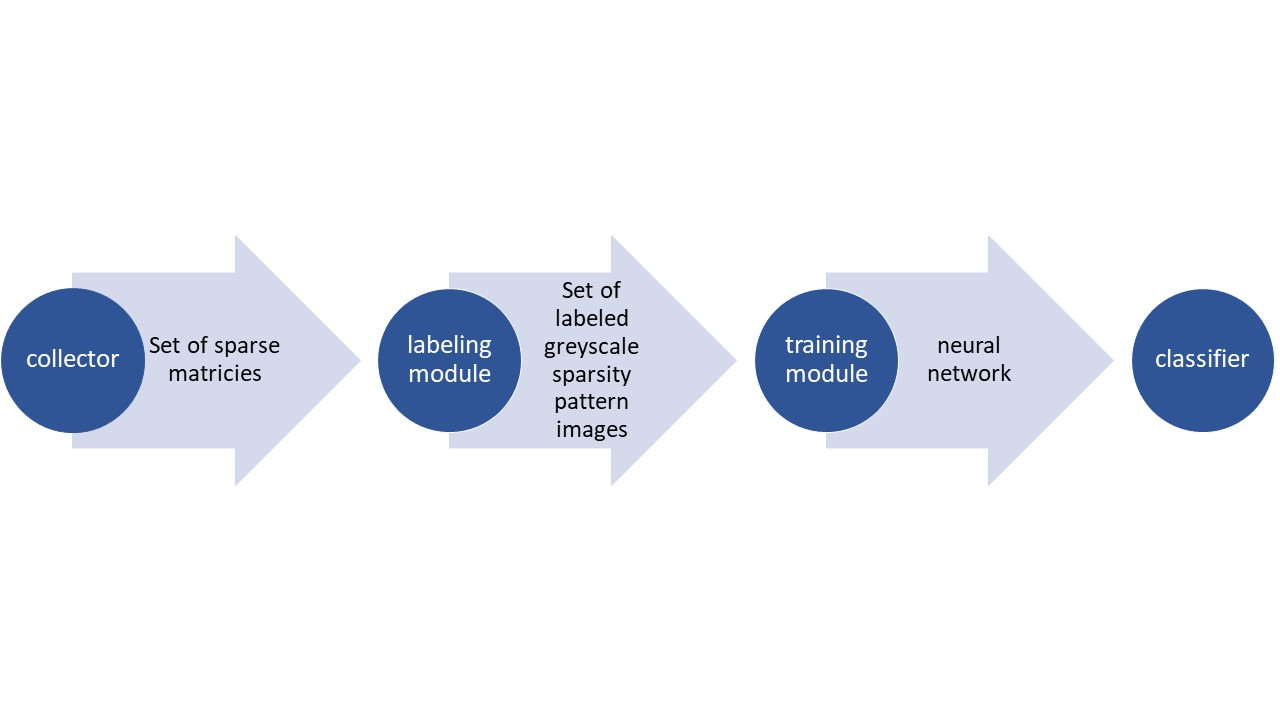
\includegraphics[width=\textwidth]{workflow}
\end{center}


\subsubsection{Use of the generator}
\textbf{Optional:} The user wants a set of matrices for his own purpose. He likes our idea of combining the creation of matrices with fetching matrices from the suite sparse matrix collection. He therefore opens the module generator. With the command generate <amount> the specified amount of matrices will be created/collected. With this command the ratio will be determined by the program. With the command create <amount> the specified amount of matrices will be created.  With the command collect <amount> the specified amount of matrices will be collected. After each command the user will be asked to specify a directory to save the matrices to.
\begin{center}
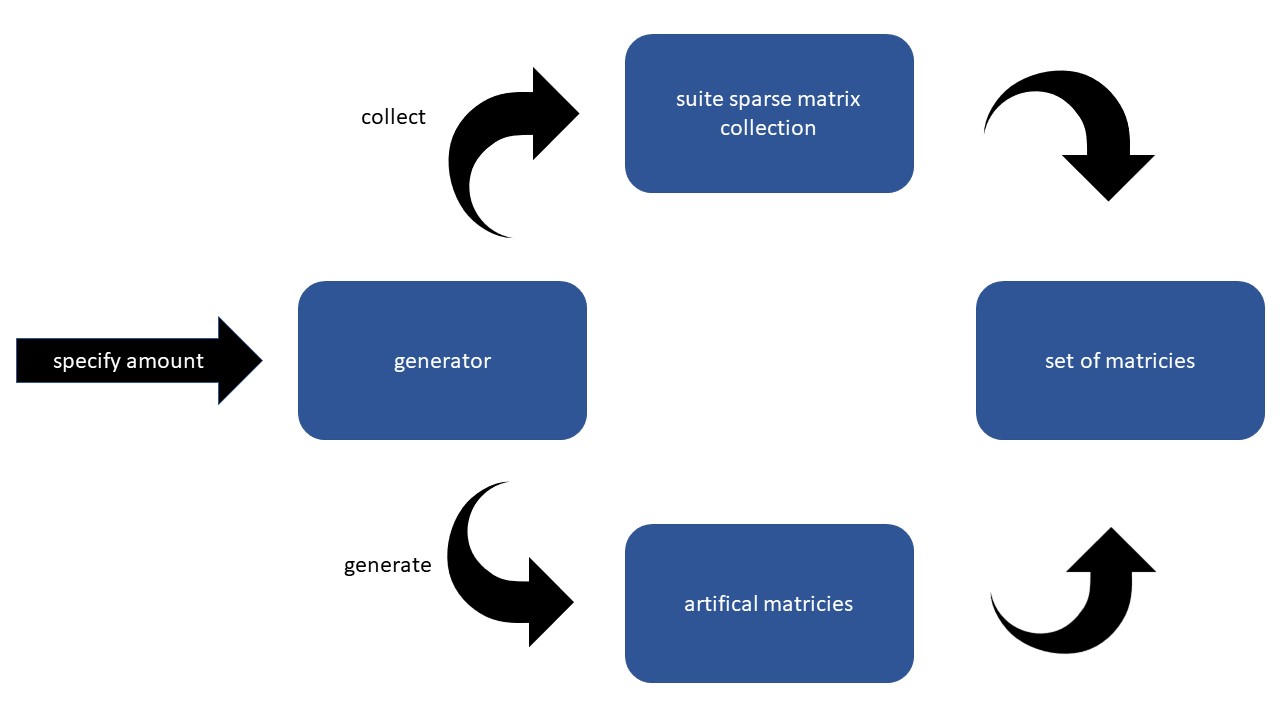
\includegraphics[width=\textwidth]{generator}
\end{center}

\subsubsection{Use of the labeling module}
\textbf{Optional:} The user has a very specific problem which generates only a certain kind of sparse matrices. That is why he wants to adapt the neural network for his specific task. He furthermore only wants to use the default preconditioner/iterative solver combinations. He first of all safes all of his matrices in one directory of his choice. Then he opens the labeling module. The command label <filepath> will label all the matrices in the directory. The user may proceed with using the neural network.


\textbf{Optional:} The user is fine with the default matrices, but he wants to use other preconditioner/iterative solver combinations which are included in the ginkgo libary. He opens the labeling module. With the command list combinations he will see all the combinations that are currently used. With the command add <preconditioner/iterative solver> a the new combinations of his choice will be added. With the command delete <preconditioner/iterative solver> the specified combination will be deleted. After the user made his choice he may proceed with using the neural network.
\begin{center}
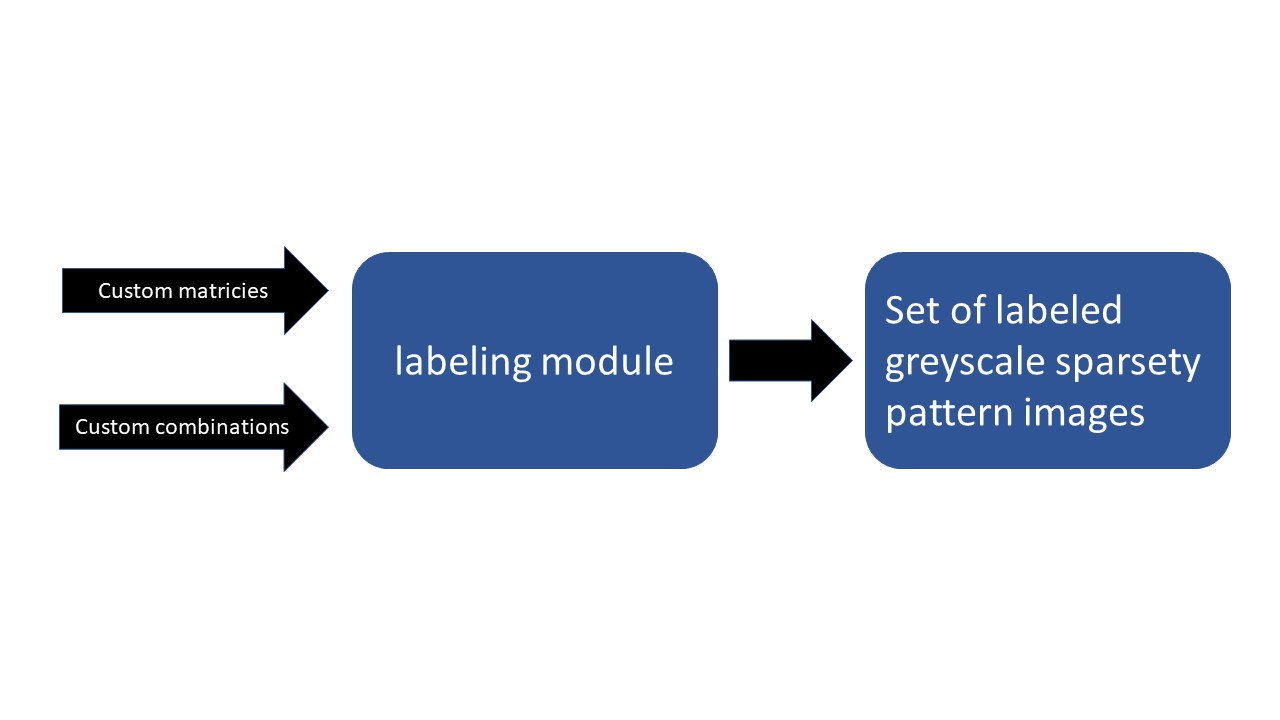
\includegraphics[width=\textwidth]{labelingModule}
\end{center}


\subsubsection{Use of the neural network}
\textbf{Optional:} The user has changed the set of matrices and/or the preconditioner/iterative solver combinations. He now wants to build the classifier. He opens the neural network module. With the command train the neural network will be trained. The user may then proceed with using the classifier.

\begin{center}
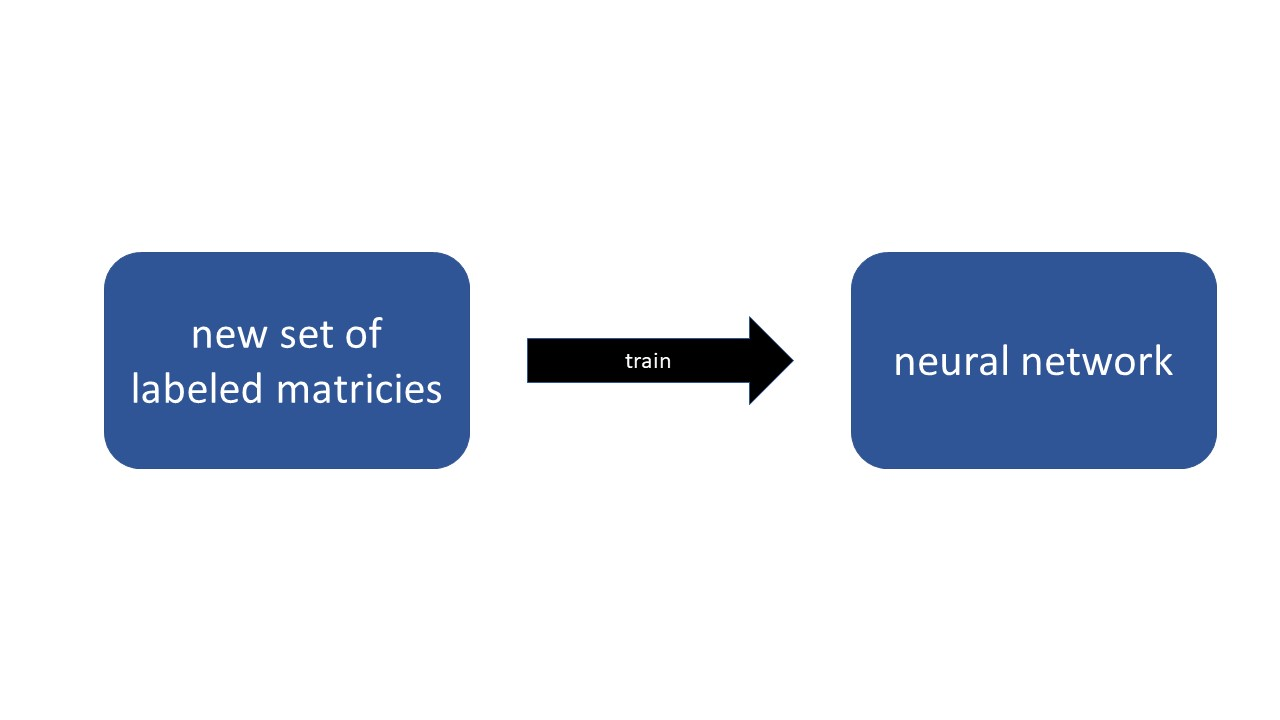
\includegraphics[width=\textwidth]{neuralNetwork}
\end{center}

\subsubsection{Use of the classifier}

The user wants to find the fastest preconditioner/iterative solver combination for a sparse linear system. If he did not change anything in the previous modules the default settings will be used. He will first save the sparse matrix in any desired filepath. Afterwards the user starts our program. The command open <filepath> loads the matrix into the program. That is when the neural network will classify the matrix and determine the fastest iterative solver/preconditioner combination for solving the matrix. This combination will be printed to the command line. (\textbf{Optional:} After determining the fastest combination the program will solve the matrix with this combination. The solved matrix will be safed in a directory the user specifies.)
\begin{center}
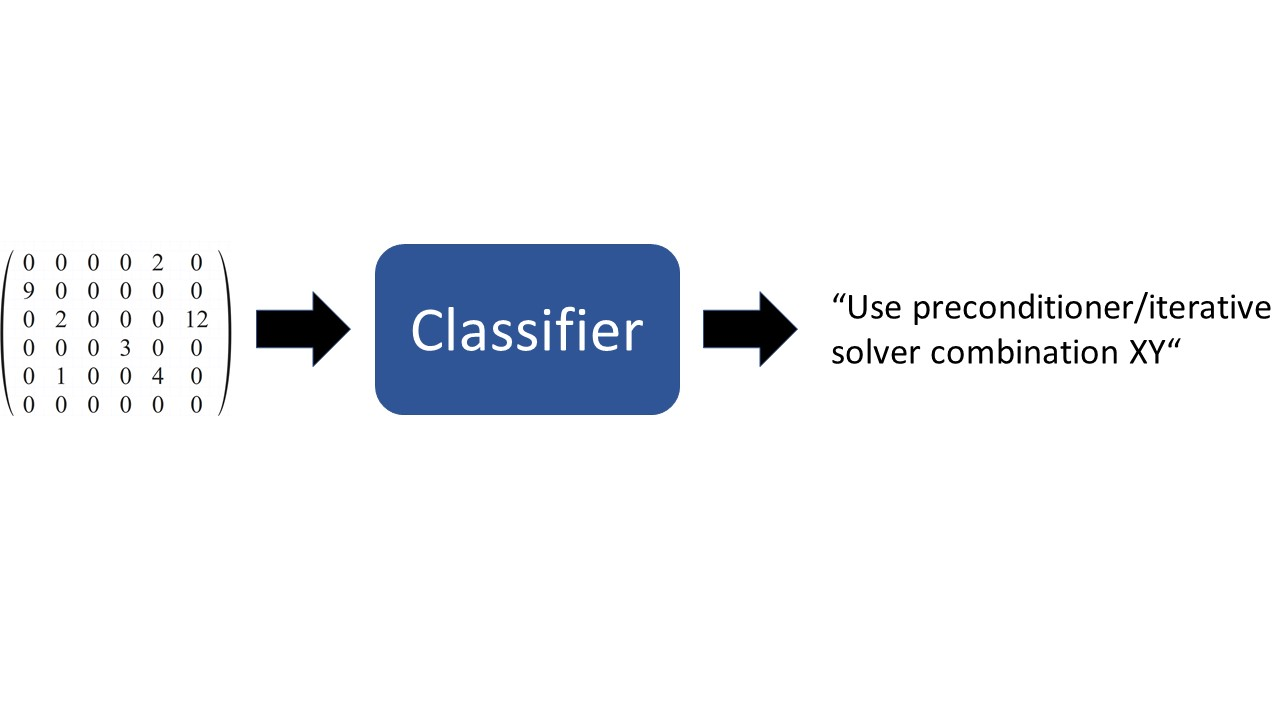
\includegraphics[width=\textwidth]{classifier}
\end{center}


\subsection{Use cases}
\subsubsection{Matrix collector}
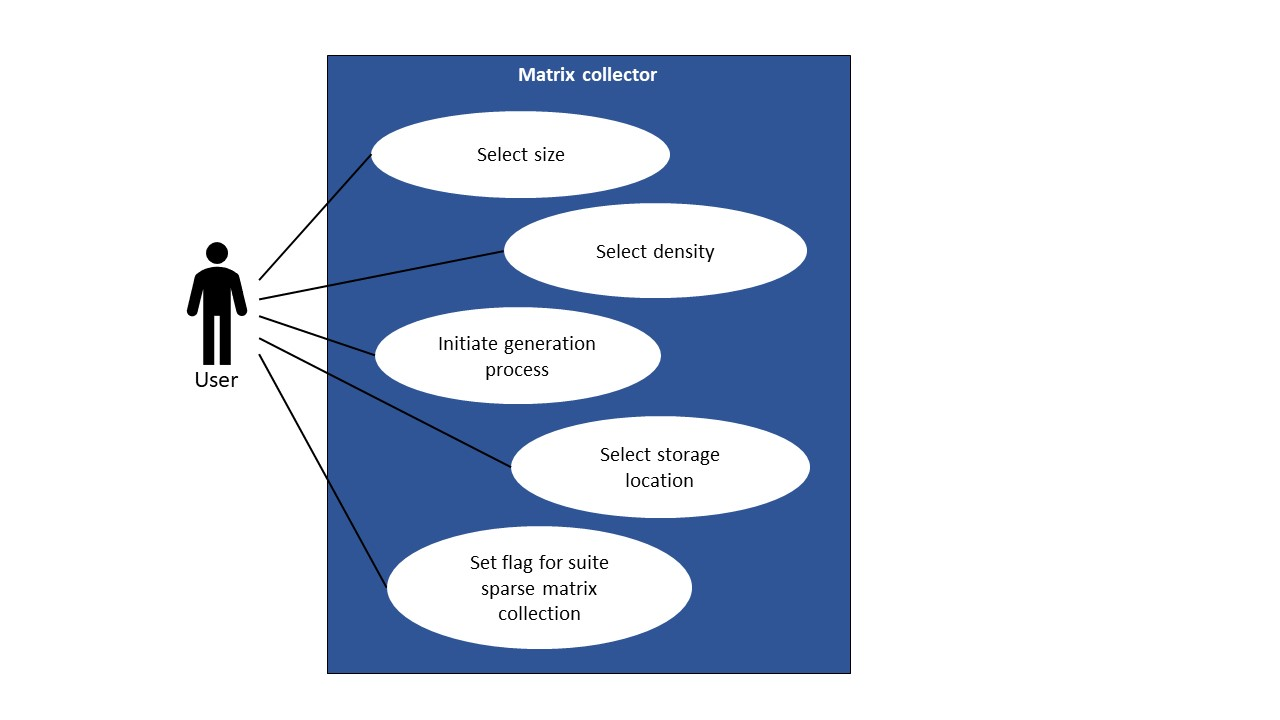
\includegraphics[width=1.3\textwidth]{useCase_Collector}
\subsubsection{Matrix labeler}
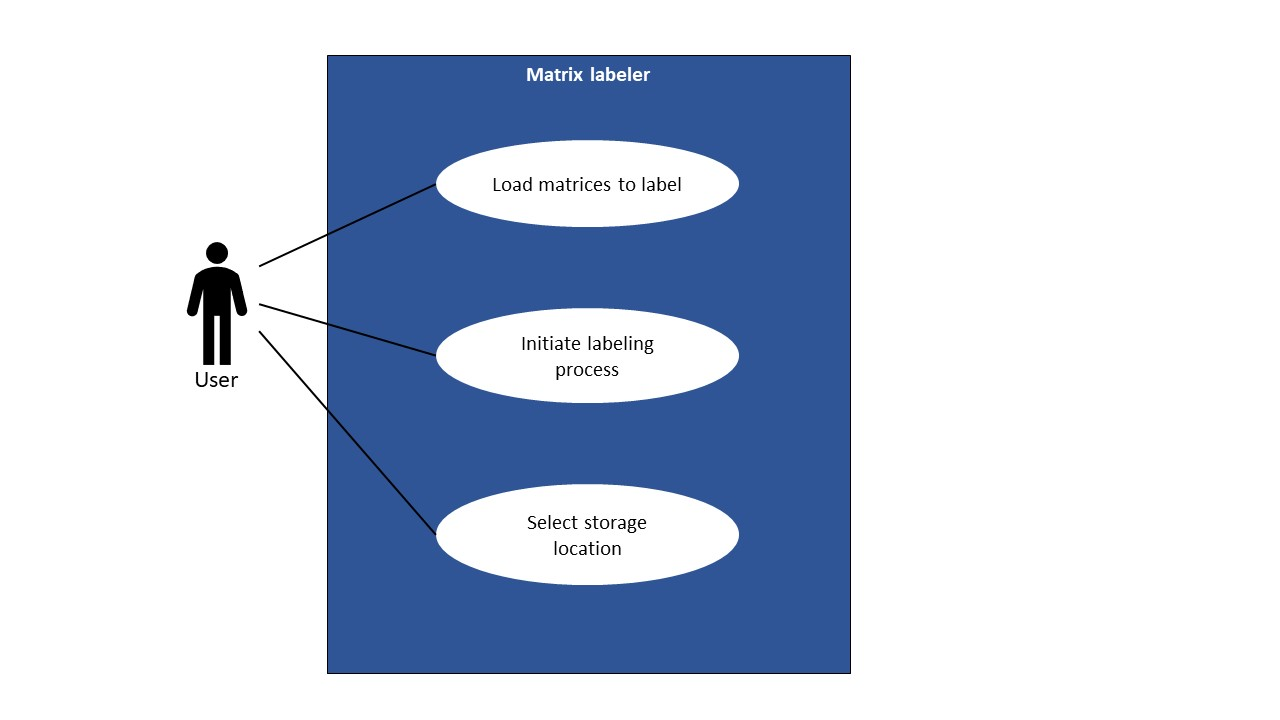
\includegraphics[width=1.3\textwidth]{useCase_Labeler}
\subsubsection{Neural network}
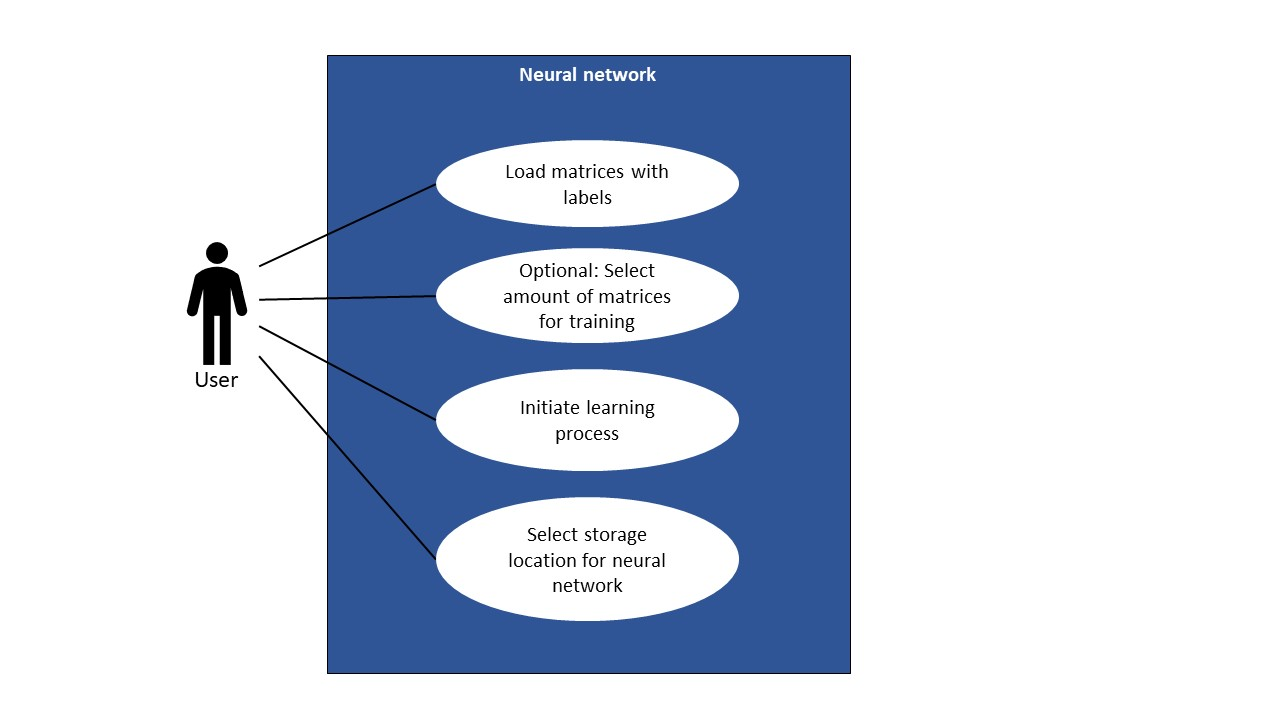
\includegraphics[width=1.3\textwidth]{useCase_NeuralNetwork}
\subsubsection{Classifier}
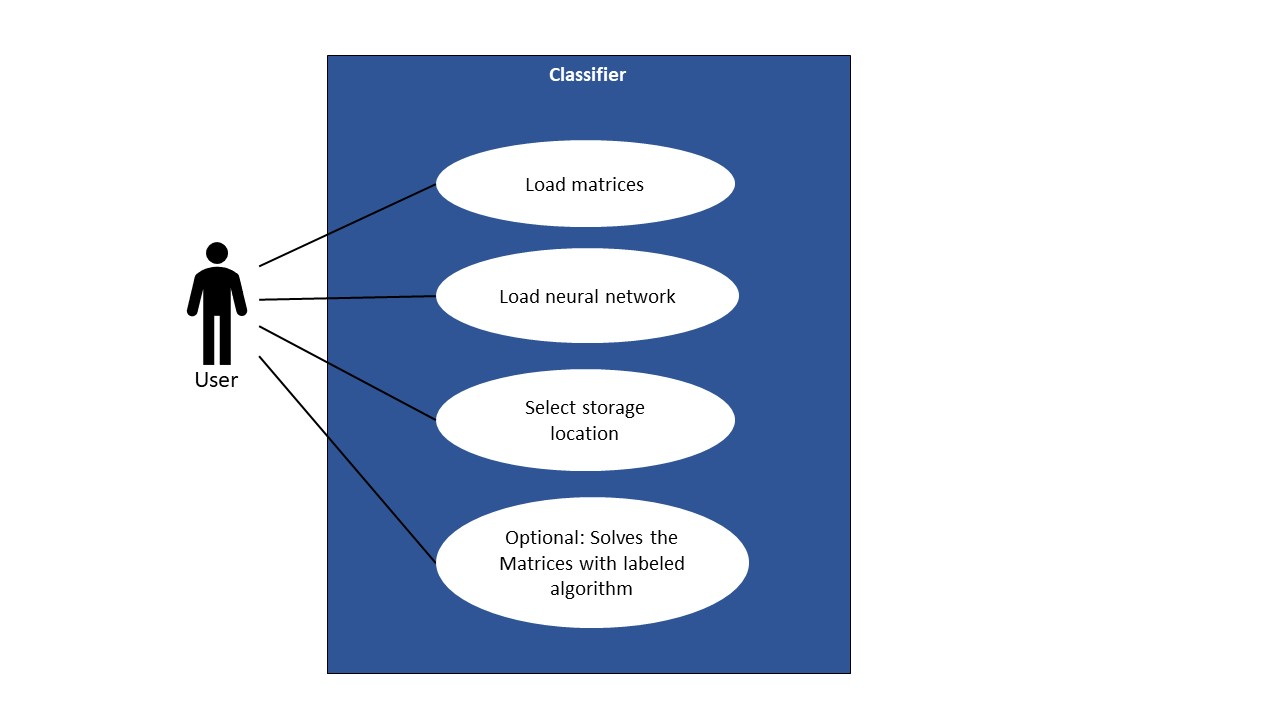
\includegraphics[width=1.3\textwidth]{useCase_Classifier}
\subsection{Object models}
\subsection{dynamic models}

\subsection{Command line options}
\begin{itemize}
\item/B10/\textbf{collect -a <amount> -n <name> -s <size> -d <density> -p <path> -g}:
\newline The user is able to create a specified amount of matrices that will be saved under a given name

\textbf{Arguments}
	\begin{itemize}
	\item[-]\textbf{-a <amount>} Absolute amount of matrices the user wants to generate
	\item[-]\textbf{-n <name>} Name under which the matrices will be saved
	\item[-]\textbf{-s <size>} (optional) Absolute size the generated square matrices should have. Default is 128
	\item[-]\textbf{-d <density>} (optional) Density level of the matrices. A float between 0 and 1 where 1 means no zero values
	\item[-]\textbf{-g}(optional) (Flag) If set it downloads as many matrices of that size as possible from the suite sparse matrix collection
	\item[-]\textbf{-g <path>} (optional) Path where the created/downloaded matrices will be saved
	\end{itemize}

\textbf{Print}
	\begin{itemize}
	\item[-]Progress notifying about the amount of matrices that are created and still need to be created
	\item[-]A message when process has finished with the path to the created matrices
	\item[-]Error, in case any required arguments are missing or invalid
	\item[-]Error, in case the specified name is already taken
	\item[-]Error, in case \textbf{-g} is set and user has no internet connection
	\item[-]Error, in case \textbf{-p <path>} is not a valid path
	\end{itemize}

\item/B20/\textbf{label -p <path> -n <name> -p <path>}:
\newline The user is able to pass matrices that he wants to get labeled

\textbf{Arguments}
	\begin{itemize}
	\item[-]\textbf{-p <path>} Absolute path to the matrices in the local storage the user wants to have labeled
	\item[-]\textbf{-n <name>} Name under which the labeled matrices will be saved
	\item[-]\textbf{-g <path>} (optional) Path where the labeled matrices will be saved
	\end{itemize}

\textbf{Print}
	\begin{itemize}
	\item[-]Progress notifying about the amount of matrices that are labeled and still need to be labeled
	\item[-]A message when process has finished with the path to the labeled matrices
	\item[-]Error, in case any required arguments are missing or invalid
	\item[-]Error, in case matrices have wrong format
	\item[-]Error, in case the specified name is already taken
	\item[-]Error, in case the remote fetching of the matrices did result in an error
	\item[-]Error, in case \textbf{-p <path>} is not a valid path
	\end{itemize}

\item/B30/\textbf{train -p <path> -n <name> -t <train> -p <path>}:
\newline The user is able to pass labeled matrices to a neural network, that will learn from this matrices

\textbf{Arguments}
	\begin{itemize}
	\item[-]\textbf{-p <path>} Absolute path to the labeled matrices on the local storage
	\item[-]\textbf{-n <name>} Name under which the neural network will be saved after training has finished
	\item[-]\textbf{-t <train>} (optional) Float between 0 and 1. Amount of matrices used for training where 1 means all. Standard is 0.8
	\item[-]\textbf{-g <path>} (optional) Path where the neural network state will be saved
	\end{itemize}

\textbf{Print}
	\begin{itemize}
	\item[-]Progress notifying about the loss of the current state based on test data
	\item[-]A message when process has finished with the path to the neural network and the final loss
	\item[-]Error, in case any required arguments are missing or invalid
	\item[-]Error, in case matrices have wrong format or are not labeled
	\item[-]Error, in case the specified name is already taken
	\item[-]Error, in case \textbf{-p <path>} is not a valid path
	\end{itemize}

\item/B40/\textbf{classify -p <path> -n <network> -s}:
\newline The user is able to pass a matrix to a the trained neural network, which will find the best solving algorithm.

\textbf{Arguments}
	\begin{itemize}
	\item[-]\textbf{-p <path>} Path to the matrix the user wants to classify
	\item[-]\textbf{-n <network>} (optional) Path to the trained neural network, if not set, uses the neural network shipped with the program
	\item[-]\textbf{-s} (optional) (Flag) If set matrix will also be solved after classification.
	\end{itemize}

\textbf{Print}
	\begin{itemize}
	\item[-]The algorithm which will be the fastest on the given matrix
	\item[-](optional) The solved matrix
	\item[-]Error, in case any required arguments are missing or invalid
	\item[-]Error, in case the matrix has a wrong format
	\item[-]Error, in case the neural network or matrix path is wrong
	\end{itemize}
\end{itemize}
\clearpage

\section{Glossar}
%generator, labeling modle, neural network, classifier, default settings  \glspl{Dateiformat}

% % Automatisch generiertes Glossar (Latex zwei mal ausführen um Glossar anzuzeigen)
%
%\glsaddall % das sorgt dafür, dass alles Glossareinträge gedruckt werden, nicht nur die verwendeten. Das sollte nicht nötig sein!
\printnoidxglossaries

\end{document}